\documentclass[12 pt ,a4 paper, openright, oneside]{article}
\setlength{\marginparwidth}{2cm}
% Pacchetti %
\usepackage[utf8]{inputenc}
\usepackage{csquotes}
\usepackage{hyperref}
\usepackage{hyphenat}
\usepackage[hypcap=true]{caption}
\usepackage{setspace}
\usepackage[hang,flushmargin,bottom]{footmisc}
\usepackage{todonotes} % Note Todo
\usepackage{soul} % strikethrough 
\usepackage{caption}
\usepackage{amssymb,amsmath}
\usepackage[official]{eurosym}
\usepackage{frontespizio}
\usepackage{subfigure}
\usepackage{float}
\usepackage{listings}
\usepackage{xcolor}
\usepackage{amsmath}
\usepackage{tabularx}
\usepackage{amsfonts} 
\usepackage[T2A,T1]{fontenc}
\usepackage[russian, english]{babel}

% Tabelle %
\usepackage[normalem]{ulem}
\useunder{\uline}{\ul}{}
\usepackage{array,ragged2e}
\usepackage{colortbl}
\newcolumntype{P}[1]{>{\RaggedRight\arraybackslash}p{#1}}

% Immagini %
\usepackage{graphicx, wrapfig, float, rotating, subfigure}

% \graphicspath{{images/}}


% Language setting
% Replace `english' with e.g. `spanish' to change the document language
\usepackage[english]{babel}
% Set page size and margins
% Replace `letterpaper' with`a4paper' for UK/EU standard size
\usepackage[letterpaper,top=2cm,bottom=2cm,left=3cm,right=3cm,marginparwidth=1.75cm]{geometry}

% Useful packages
\usepackage{amsmath}
\usepackage{graphicx}
\usepackage{float}
\usepackage{hyperref}

\begin{document}
\include{frontespizio.tex}
\tableofcontents
\include{intro.tex}
\section{Information Visualization}
La visualizzazione delle informazioni è un modo per comunicare significativamente i dati e aiutare le persone a 
dare un senso a grandi quantità di informazioni.
Le visualizzazioni come artefatti cognitivi che consentono il trattamento parallelo delle informazioni.
Tre scopi principali della visulizzazione:
\begin{itemize}
    \item \textbf{Explanatory}: Le visualizzazioni esplicative sono strumenti per presentare informazioni, comunicare dati e messaggi, spiegare qualcosa a qualcun altro.
    \item \textbf{Exploratory}: Le visualizzazioni esplorative sono strumenti per i lettori per analizzare ciò che viene loro presentato. Molto spesso, l'esito dell'analisi esplorativa non è solo la risposta alle domande originali, ma la generazione di nuove domande.
    \item \textbf{Confirmatory}: Nell'analisi confermativa, le visualizzazioni sono destinate a testare ipotesi.
\end{itemize}

Bisogna decidere cosa visualizzare 
\begin{figure}[H]
    \centering
    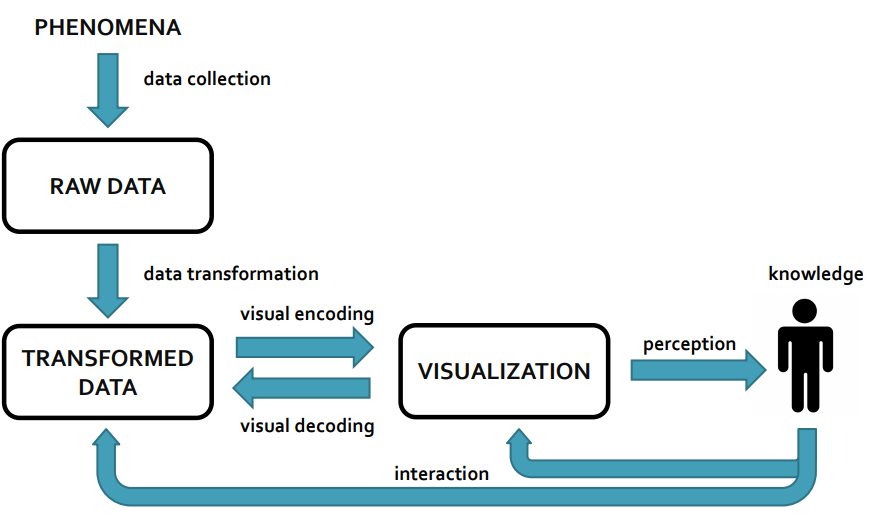
\includegraphics[width=0.5\textwidth]{images/visPipe2.png} % Sostituisci 'nome_immagine' con il nome del tuo file immagine
    \caption{Visualization pipeline}
    \label{fig:immagine}
\end{figure}
\subsection{Data}
Informazioni fattuali come misurazioni o statistiche, utilizzate come base per il ragionamento, la discussione o il calcolo.
I dati sono collezioni di \textit{items} e \textit{attributes} degli items.
Gli \textit{Items} sono gli oggetti/entità che vogliamo viusalizzare.
Gli \textit{Attributi} sono le proèrietà degli oggetti/entità.

Una \textit{Tabella} è una griaglia di colonne e righr, dove le righe  rapresentanto gli item e le colonne gli attributi.
Un \textit{network} è una collezione di nodi che rappresentano gli item, connessi tramite dei link; entrambi nodi e link possono avere attributi.

\subsection{Tipi di attributi}
\begin{itemize}
    \item \textit{Quantitativi}: sono gli attributi dove i valori rappresentano quantità misurate, 
        questi valori possono essere ordinati, ma può essere calcolata anche la distanza tra i valori.
    \item  \textit{Categorici}: sono gli attributi dove i valori descrivino le categorie,
        possono essere di tre tipi, \textbf{Nominali} se non hanno un ordine particolare, \textbf{Ordinali} se possono essere ordinati,
        \textbf{Binary} se hanno solo due stati.
\end{itemize}
\subsection{Semantica degli attributi}
\begin{itemize}
    \item \textbf{Spaziali e temporali}: Esempio la location, latitudine e longitudine o la data di assunzione come attributo temporale.
    \item \textbf{Sequnziali, ciclici divergenti}: Esempio: i mesi dell'anno sono ciclici, la temperatura è un attributo divergente.
    \item \textbf{Gerarchici}: Tipi di prodotto con sottocategorie, un esempio sono i vestiti.
\end{itemize}
Si deve selezionare la visualizzazione appropriata a seconda del tipo e dalla semantica dell'attributo.
Esempio:
\begin{figure}[H]
    \centering
    \begin{minipage}{0.45\textwidth}
        \centering
        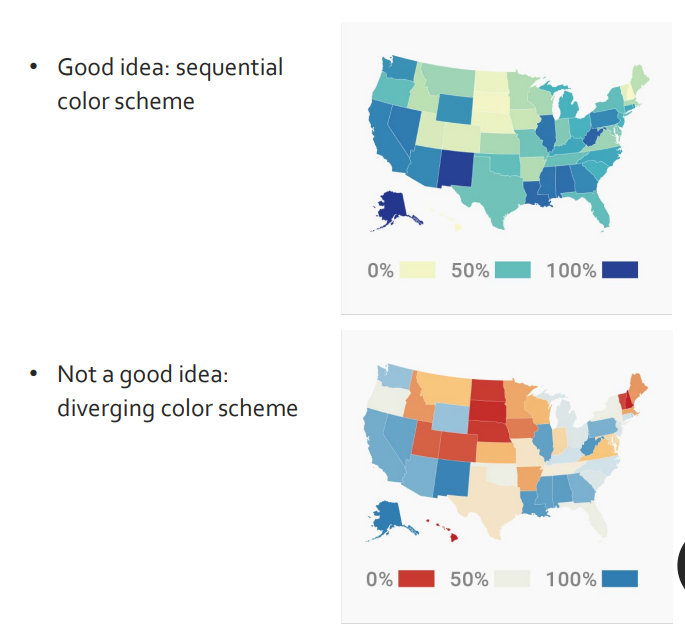
\includegraphics[width=\linewidth]{images/Attrubtevis.png} 
        \caption{Differenza di Visualizzazione}
        \label{fig:immagine1}
    \end{minipage}\hfill
    \begin{minipage}{0.45\textwidth}
        \centering
        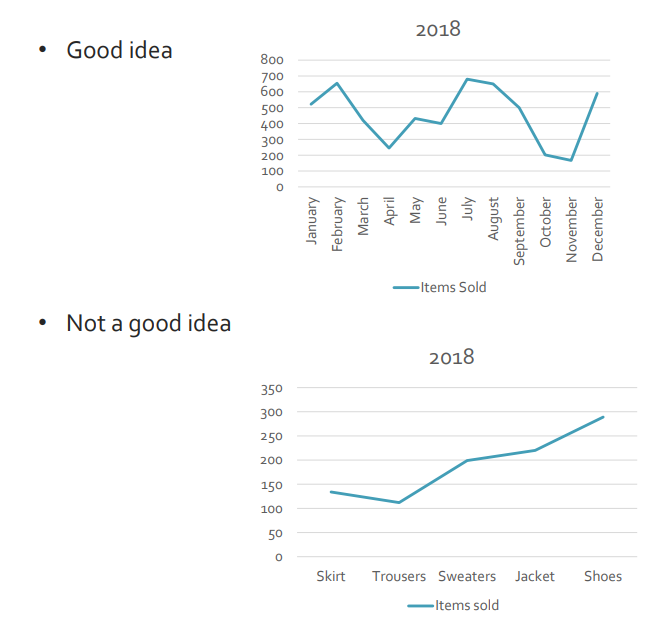
\includegraphics[width=\linewidth]{images/Attributevis2.png} % Sostituisci 'immagine2' con il nome del tuo file immagine
        \caption{Differenza di Visualizzazione}
        \label{fig:immagine2}
    \end{minipage}
\end{figure}
\subsection{Grafici Fondamentali (Bivariate data)} %--------------------------------------------------------------------------


\subsubsection{Bar Charts}
Visualizza come una quantità misurata si distribuisce tra categorie. Ogni barra rappresenta una categoria e la lunghezza della barra è una quantità misurata in quella categoria. Dati bivariati: nominale/ordinale e quantitativo.
 Non confondere con gli istogrammi
\begin{figure}[H]
    \centering
    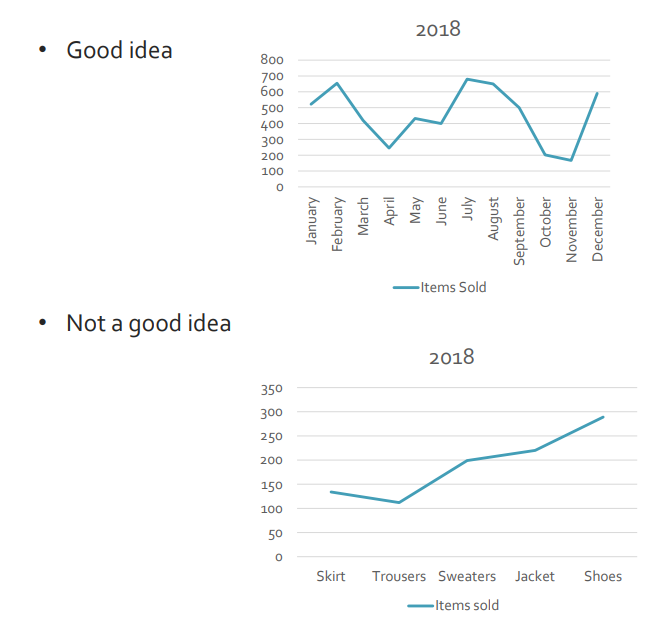
\includegraphics[width=0.5\textwidth]{images/BarCharts.png} 
    \caption{Bar Charts}
    \label{fig:immagine}
\end{figure}
\subsubsection{Histograms}
Frequenza degli elementi. Dati bivariati: una variabile indipendente quantizzata in intervalli 
(blocchi) e una variabile dipendente.
\begin{figure}[H]
    \centering
    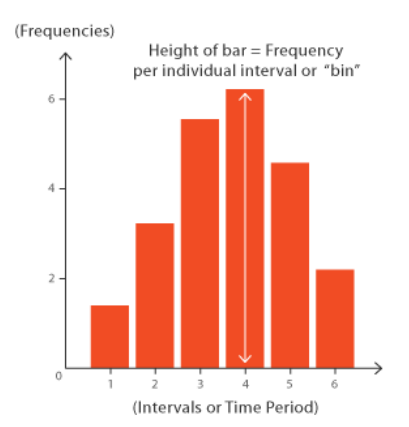
\includegraphics[width=0.5\textwidth]{images/Histograms.png} 
    \caption{Histograms}
    \label{fig:immagine}
\end{figure}
\subsubsection{Pie Charts}
Mostrare proporzioni e percentuali tra le categorie. Utile per dare un'idea rapida e confrontare una fetta rispetto al totale, non adatto per confronti accurati. Altri svantaggi: numero limitato di valori, 
occupazione dello spazio.
\begin{figure}[H]
    \centering
    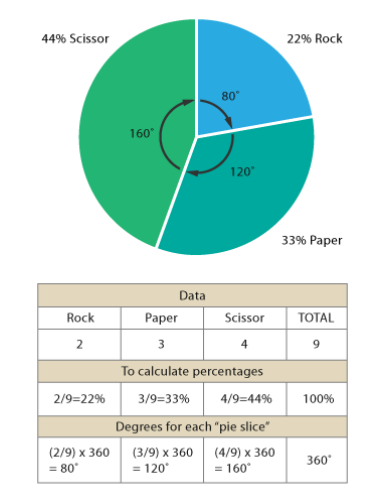
\includegraphics[width=0.5\textwidth]{images/PieChart.png} 
    \caption{Pie Charts}
    \label{fig:immagine}
\end{figure}

\subsubsection{Donut Charts}
Grafici a torta con l'area centrale tagliata. Maggiore enfasi sulla lunghezza dell'arco rispetto all'area. 
Più efficienti in termini di spazio.
\begin{figure}[H]
    \centering
    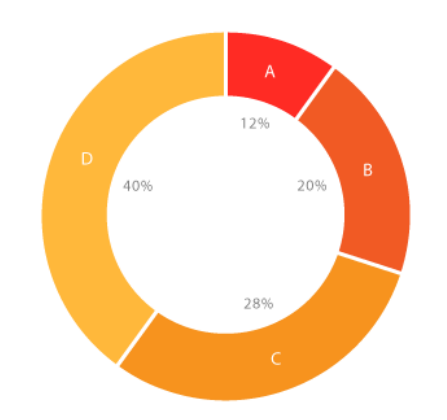
\includegraphics[width=0.5\textwidth]{images/DonutCharts.png} % Sostituisci 'nome_immagine' con il nome del tuo file immagine
    \caption{Donut Charts}
    \label{fig:immagine}
\end{figure}
\subsubsection{Scatter plots}
Relazione tra attributi: visualizzazione di come una quantità è correlata a un'altra 
(e analisi di cluster, valori anomali, ecc.). Dati bivariati: 
due attributi quantitativi indipendenti.
\begin{figure}[H]
    \centering
    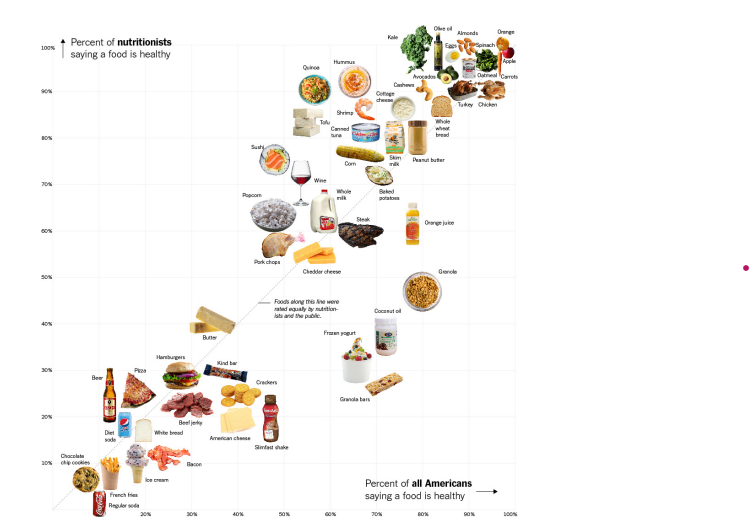
\includegraphics[width=0.5\textwidth]{images/ScatterPlots.png} % Sostituisci 'nome_immagine' con il nome del tuo file immagine
    \caption{Scatter plots}
    \label{fig:immagine}
\end{figure}
\subsubsection{Slope Charts}
Alternativa ai Scatter plots: assi paralleli, ogni elemento è una linea che collega due quantità.
\begin{figure}[H]
    \centering
    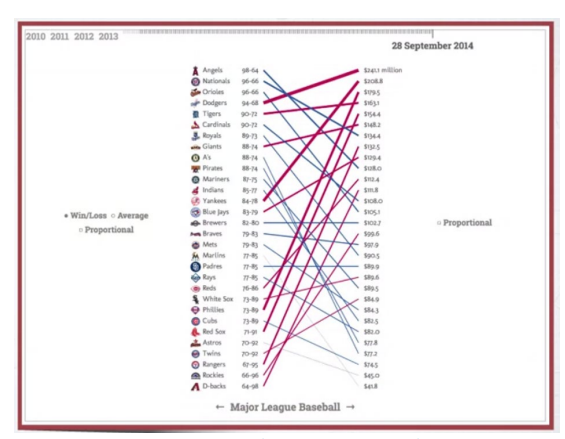
\includegraphics[width=0.5\textwidth]{images/SlopeCharts.png} 
    \caption{Slope Charts}
    \label{fig:immagine}
\end{figure}
\subsubsection{Line Charts}
\begin{figure}[H]
    \centering
    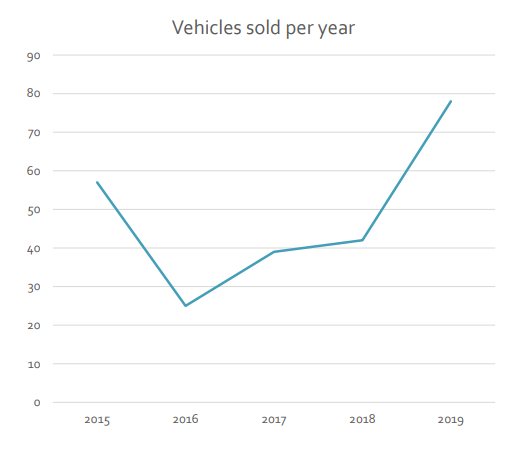
\includegraphics[width=0.5\textwidth]{images/LineCharts.png}
    \caption{Line Charts}
    \label{fig:immagine}
\end{figure}
\subsubsection{Area Charts}
Line Charts dove l'area sotto alla linea è riempita.
\begin{figure}[H]
    \centering
    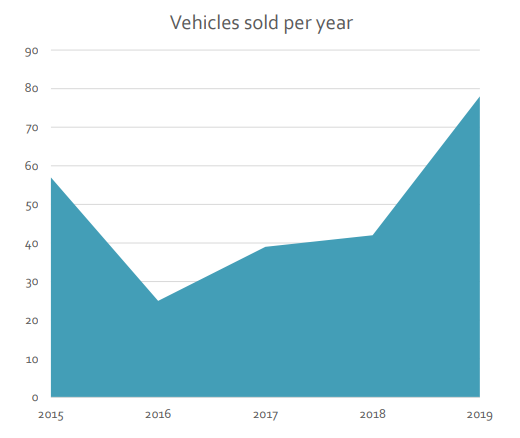
\includegraphics[width=0.5\textwidth]{images/AreaCharts.png}
    \caption{Area Charts}
    \label{fig:immagine}
\end{figure}
\subsubsection{Chropleth maps}
Come si distribuisce una quantità nelle diverse aree/geografiche/regioni. Colori, sfumature, pattern sono utilizzati per rappresentare la quantità associata alle aree/regioni. Buona panoramica (ma non confronto accurato). Rischio: 
confondere l'area geografica con i valori dei dati (prestare attenzione alla normalizzazione).
\begin{figure}[H]
    \centering
    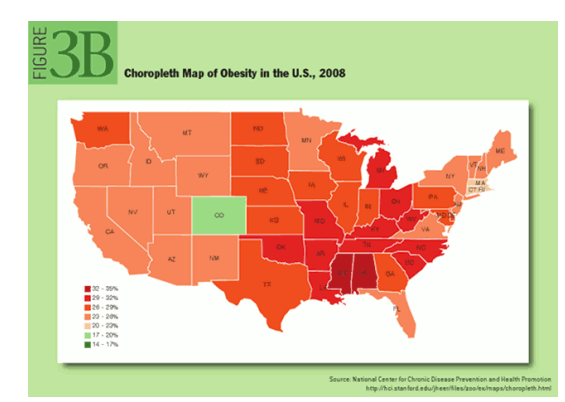
\includegraphics[width=0.5\textwidth]{images/Chropolet.png} 
    \caption{Chropleth maps}
    \label{fig:immagine}
\end{figure}
\subsubsection{Symbol maps}
Come si distribuisce una quantità lungo due coordinate spaziali. Un simbolo (spesso un disco o un quadrato) è posizionato 
in un punto e dimensionato in modo che la sua area sia proporzionale alla quantità associata al punto.
\begin{figure}[H]
    \centering
    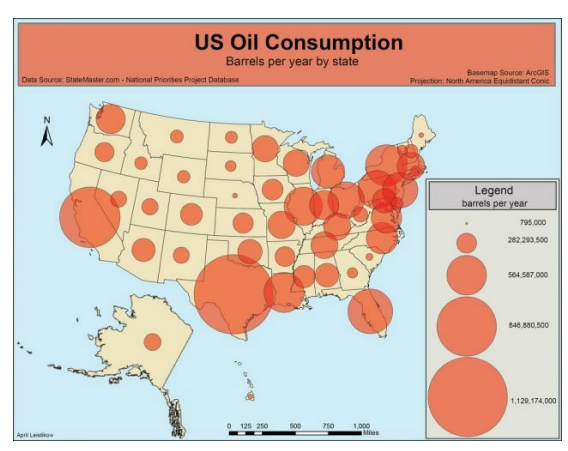
\includegraphics[width=0.5\textwidth]{images/SymbolMaps.png} 
    \caption{Symbol maps}
    \label{fig:immagine}
\end{figure}

\subsection{Grafici Fondamentali (Attributi Multipli)}
\subsubsection{Stacked Bar Charts}
\begin{figure}[H]
    \centering
    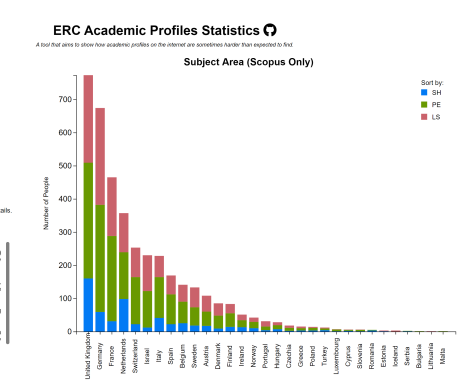
\includegraphics[width=0.5\textwidth]{images/StackedBar.png} % Sostituisci 'nome_immagine' con il nome del tuo file immagine
    \caption{Stacked Bar Charts}
    \label{fig:immagine}
\end{figure}
\subsubsection{Grouped Bar Charts}
\begin{figure}[H]
    \centering
    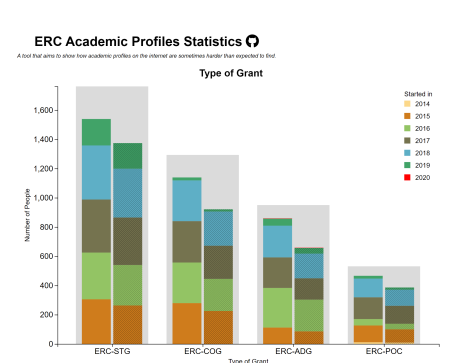
\includegraphics[width=0.5\textwidth]{images/GroupedBar.png} % Sostituisci 'nome_immagine' con il nome del tuo file immagine
    \caption{Grouped Bar Charts}
    \label{fig:immagine}
\end{figure}
\subsubsection{Stacked Line Charts}
\begin{figure}[H]
    \centering
    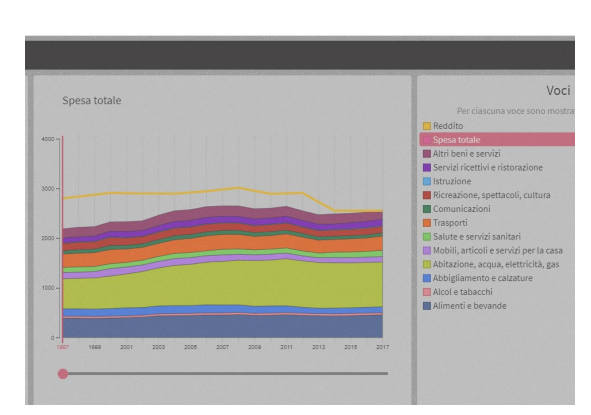
\includegraphics[width=0.5\textwidth]{images/Stacked.png} % Sostituisci 'nome_immagine' con il nome del tuo file immagine
    \caption{Stacked Line Charts}
    \label{fig:immagine}
\end{figure}
\subsubsection{Line Charts Series}
\begin{figure}[H]
    \centering
    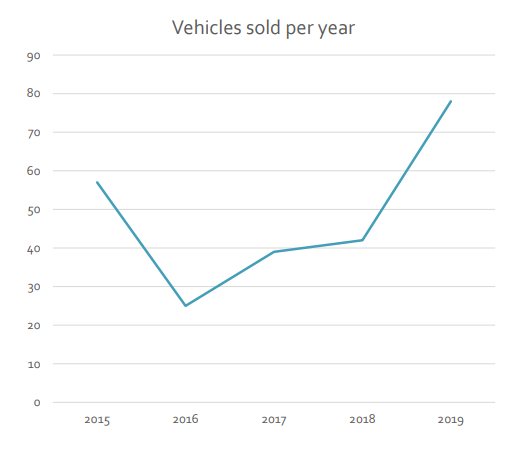
\includegraphics[width=0.5\textwidth]{images/LineCharts.png} % Sostituisci 'nome_immagine' con il nome del tuo file immagine
    \caption{Line Charts Series}
    \label{fig:immagine}
\end{figure}
\subsubsection{Bubble Charts}
\begin{figure}[H]
    \centering
    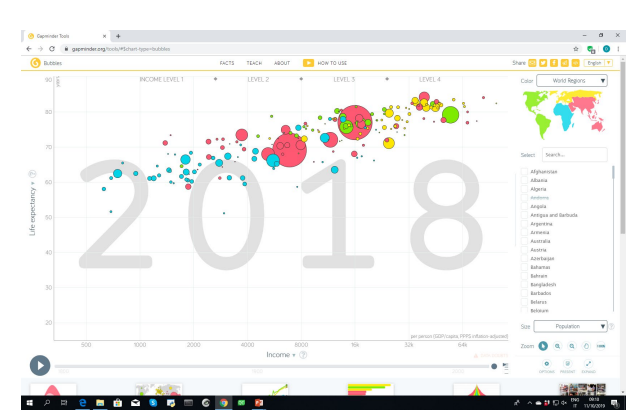
\includegraphics[width=0.5\textwidth]{images/Bubble.png} % Sostituisci 'nome_immagine' con il nome del tuo file immagine
    \caption{Bubble Charts}
    \label{fig:immagine}
\end{figure}
\subsubsection{Small multiples}
\begin{figure}[H]
    \centering
    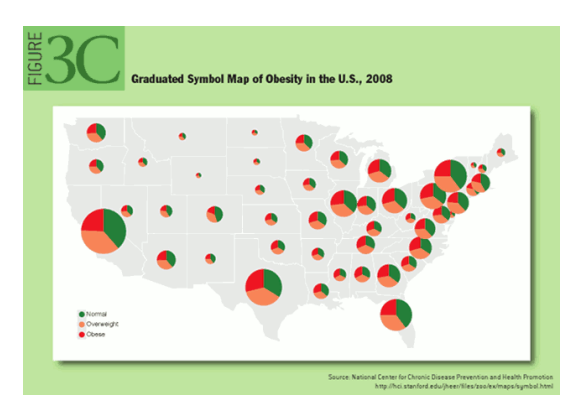
\includegraphics[width=0.5\textwidth]{images/SmallMultiples2.png} % Sostituisci 'nome_immagine' con il nome del tuo file immagine
    \caption{Small multiples}
    \label{fig:immagine}
\end{figure}
\subsubsection{Symbol Maps}
\begin{figure}[H]
    \centering
    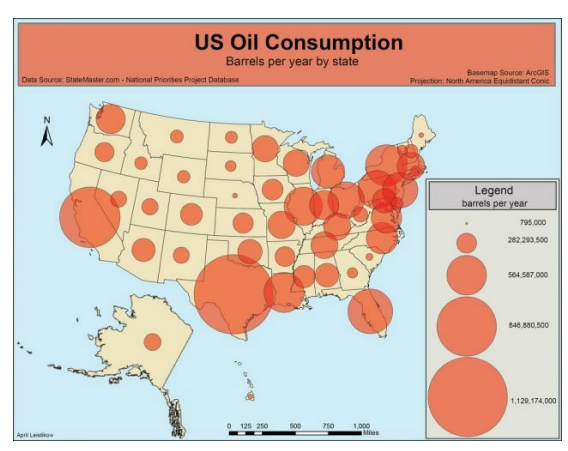
\includegraphics[width=0.5\textwidth]{images/SymbolMaps.png} % Sostituisci 'nome_immagine' con il nome del tuo file immagine
    \caption{Symbol Maps}
    \label{fig:immagine}
\end{figure}
\subsection{Grafici Fondamentali (Attributi Gerarchici)}
\subsubsection{Sunburst Charts}
\begin{figure}[H]
    \centering
    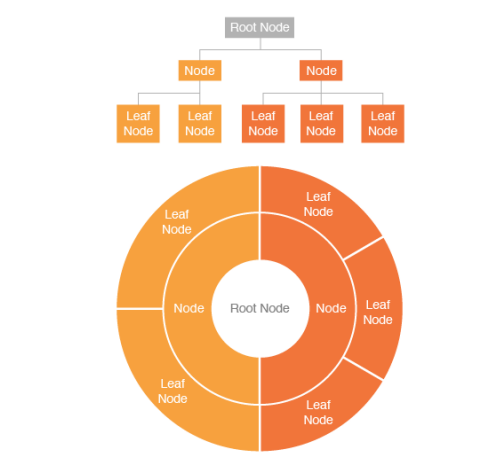
\includegraphics[width=0.5\textwidth]{images/SunBurst.png} % Sostituisci 'nome_immagine' con il nome del tuo file immagine
    \caption{Sunburst Charts}
    \label{fig:immagine}
\end{figure}
\subsubsection{Treempas}
\begin{figure}[H]
    \centering
    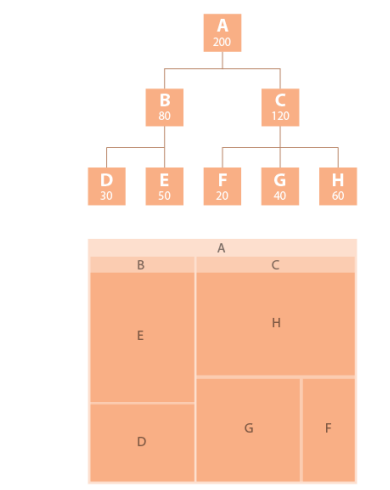
\includegraphics[width=0.5\textwidth]{images/TreeMpas.png} % Sostituisci 'nome_immagine' con il nome del tuo file immagine
    \caption{Treempas}
    \label{fig:immagine}
\end{figure}
\section{Information Visualization II}
\subsection{Visual Encoding}
Le visualizzazioni sono composte da \textbf{marks} (segnali) e 
\textbf{channels} (canali). I marks sono gli oggetti grafici che rappresentano gli elementi di dati (ad esempio, punti, linee, barre).
I channels sono le proprietà grafiche che rappresentano gli attributi dei dati (ad esempio, colore, posizione, forma, dimensione).


La codifica visiva significa passare dai dati alle rappresentazioni visive.
La codifica richiede non solo la scelta di un grafico appropriato per i dati in questione (tipo e semantica),
ma anche la selezione degli elementi grafici individuali e delle loro proprietà.

\subsection{Graphical Elements}
\begin{figure}[H]
    \centering
    \begin{minipage}{0.45\textwidth}
        \centering
        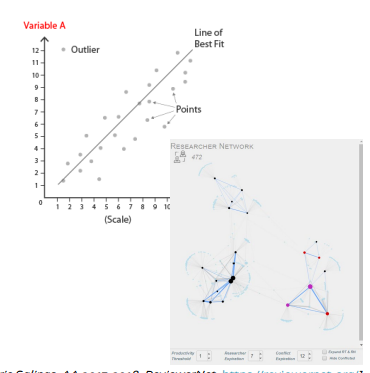
\includegraphics[width=\linewidth]{images/Marks.png} 
        \caption{Esempio di Marks}
        \label{fig:immagine1}
    \end{minipage}\hfill
    \begin{minipage}{0.45\textwidth}
        \centering
        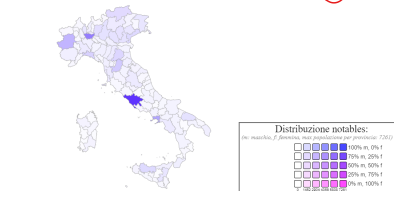
\includegraphics[width=\linewidth]{images/Channels.png} % Sostituisci 'immagine2' con il nome del tuo file immagine
        \caption{Esempio di Channels}
        \label{fig:immagine2}
    \end{minipage}
\end{figure}
Le componenti contestuali sono elementi che rendono più semplice interpretare le visualizzazioni.
Un esempio sono: le labesls, annotazioni, legende, griglie, assi cartesiani.
\begin{figure}[H]
    \centering
    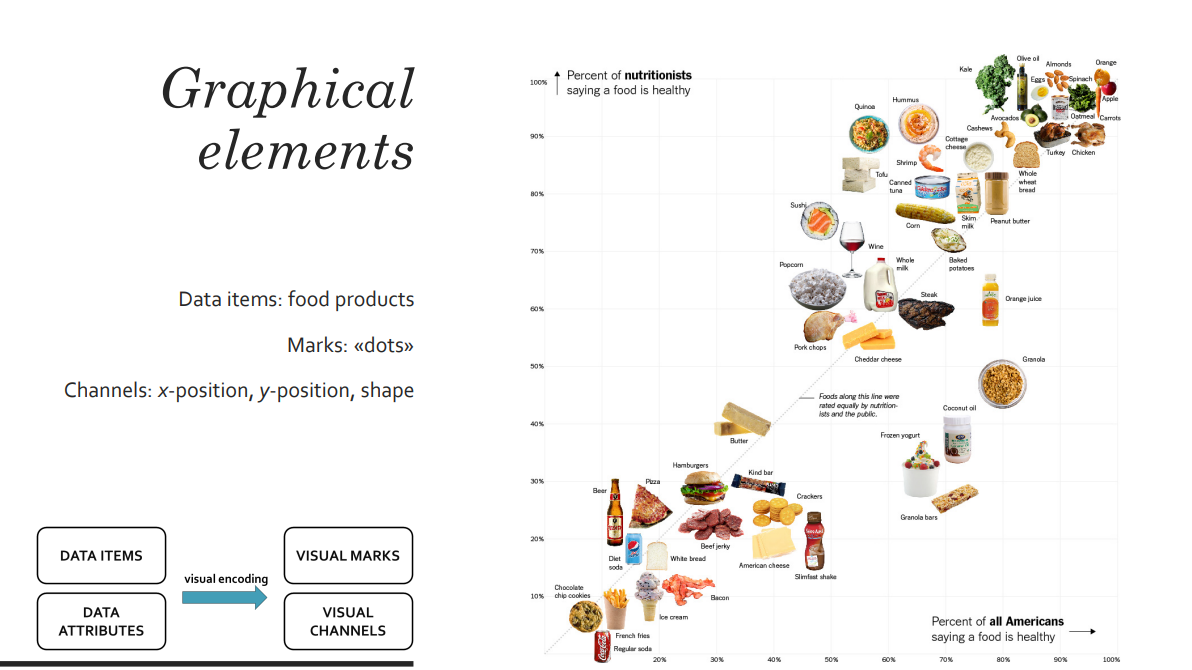
\includegraphics[width=0.5\textwidth]{images/CompleteExMC.png} % Sostituisci 'nome_immagine' con il nome del tuo file immagine
    \caption{Esempio completo di Channels e Marks di un grafico}
    \label{fig:immagine}
\end{figure}
\subsection{Visual decoding}
\begin{figure}[H]
    \centering
    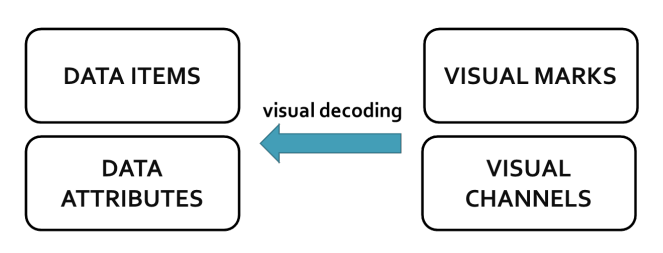
\includegraphics[width=0.5\textwidth]{images/VisDec.png} % Sostituisci 'nome_immagine' con il nome del tuo file immagine
    \caption{Visual Decoding}
    \label{fig:immagine}
\end{figure}
Per \textbf{Visual Decoding} si intende destrutturare una rappresentazione visiva nei suoi principali elementi e identificare:
\begin{itemize}
    \item gli elementi grafici, quali sono i segnali visivi? Quali sono i canali visivi?
    \item le regole di mappatura (ossia, le informazioni che i singoli elementi grafici rappresentano)
        quali elementi di dati rappresentano i segnali? Quali attributi rappresentano i canali?
\end{itemize}
È utile per valutare e ridisegnare le visualizzazioni.

\begin{figure}[H]
    \centering
    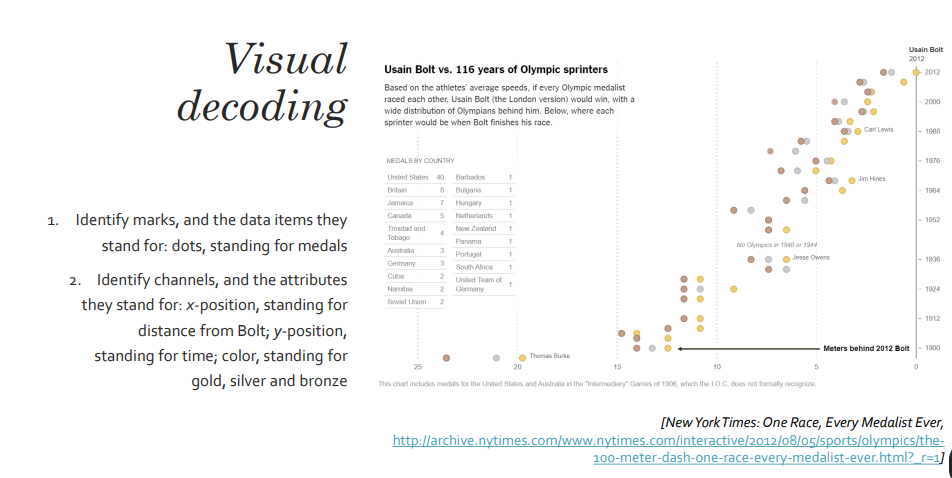
\includegraphics[width=0.5\textwidth]{images/ExComplDec.png} % Sostituisci 'nome_immagine' con il nome del tuo file immagine
    \caption{Esempio completo di Decoding}
    \label{fig:immagine}
\end{figure}

\subsubsection{Quality Evaluation}
La valutazione di una visualizzazione può basarsi su due principi 
guida principali: \textbf{Expressiveness} ed \textbf{Effectiveness}.
\textbf{Expressiveness}: la Visual representation dovrebbe rappresentare tutte e solo le relazioni che esistono nei dati.
Le informazioni rilevanti dovrebbero essere prioritarie e quindi codificate con i canali più efficaci/accurati.
\begin{figure}[H]
    \centering
    \begin{minipage}{0.45\textwidth}
        \centering
        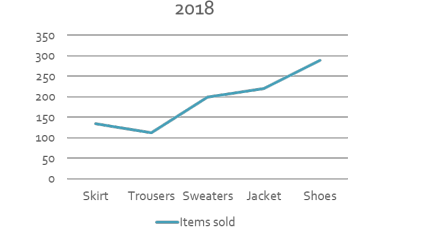
\includegraphics[width=\linewidth]{images/ErroreEff.png} 
        \caption{Dati non ordinati che sembrano ordinati (nell'esempio seguente, stiamo mostrando informazioni su un trend che non è nei dati:
         la forma della linea non ha significato).}
        \label{fig:immagine1}
    \end{minipage}\hfill
    \begin{minipage}{0.45\textwidth}
        \centering
        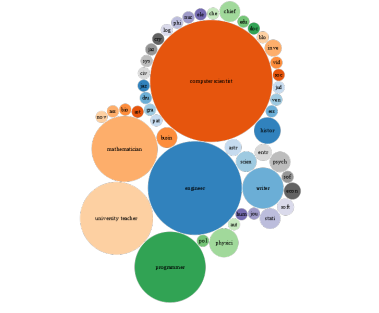
\includegraphics[width=\linewidth]{images/ErroreEff2.png} % Sostituisci 'immagine2' con il nome del tuo file immagine
        \caption{utilizzo dei colori quando non restituiscono alcuna informazione}
        \label{fig:immagine2}
    \end{minipage}
\end{figure}
\subsubsection{Percentuale di Accuracy}
Quanto sono efficaci i canali nel trasmettere diversi tipi di attributi?
Uno dei (possibili) riassunti per attributi quantitativi.
\begin{figure}[H]
    \centering
    \begin{minipage}{0.45\textwidth}
        \centering
        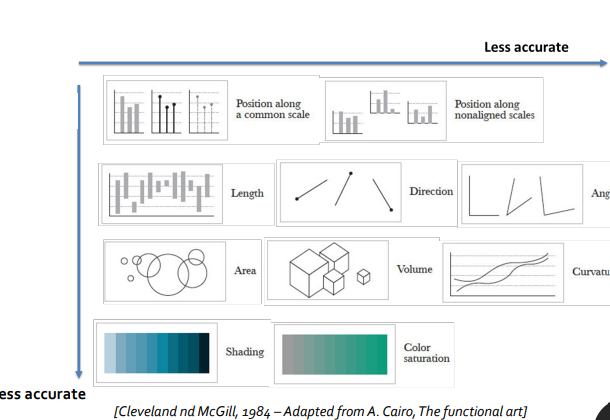
\includegraphics[width=\linewidth]{images/percentAcc1.png} 
        \caption{Riassunto dell'accuracy di ogni grafico.}
        \label{fig:immagine1}
    \end{minipage}\hfill
    \begin{minipage}{0.45\textwidth}
        \centering
        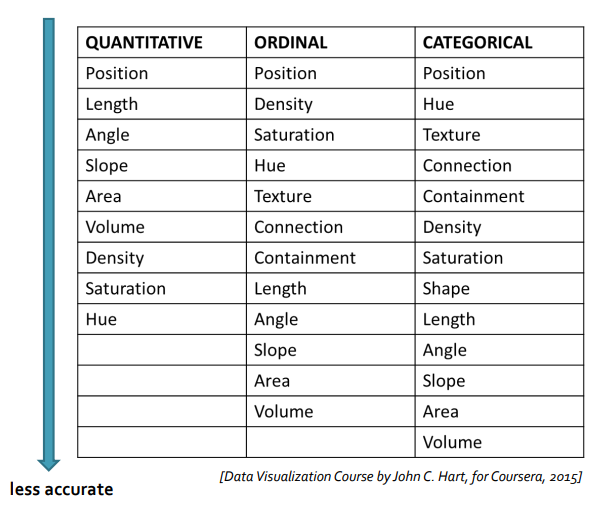
\includegraphics[width=\linewidth]{images/percentAcc2.png} 
        \caption{Riassunto dell'accuracy di ogni grafico}
        \label{fig:immagine2}
    \end{minipage}
\end{figure}
\subsection{Altri tipi di grafici}
\subsubsection{WordClouds}
Rappresentazione di quanto frequentemente le parole appaiono in un determinato corpo di testo attraverso la dimensione della parola
Variazioni nell'arrangiamento e nel colore
Principalmente utilizzato per motivi estetici.
\begin{figure}[H]
    \centering
    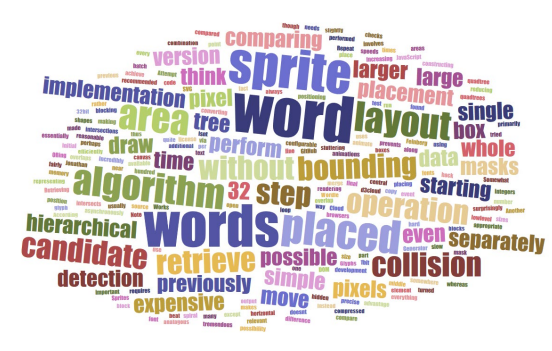
\includegraphics[width=0.5\textwidth]{images/WordClouds.png} 
    \caption{WordClouds}
    \label{fig:immagine}
\end{figure}
\subsubsection{Calligrams}
Testi disposti in modo tale da formare un'immagine tematicamente correlata.
L'immagine creata dalle parole illustra il testo esprimendo visivamente qualcosa associato (o in contrasto) a ciò che il testo dice.
\begin{figure}[H]
    \centering
    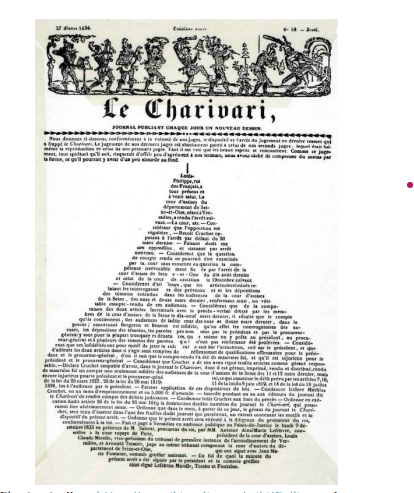
\includegraphics[width=0.5\textwidth]{images/Calligrams.png} 
    \caption{Calligrams}
    \label{fig:immagine}
\end{figure}

\subsubsection{Flow Maps}

Raffigurare il movimento delle entità posizionando linee tracciate sopra delle mappe (spazio e tempo)
Lo spessore, il colore, ecc. possono codificare informazioni aggiuntive
In questa mappa: dimensioni delle truppe, distanza percorsa, temperatura, latitudine e longitudine, direzione del viaggio, tempo.
\begin{figure}[H]
    \centering
    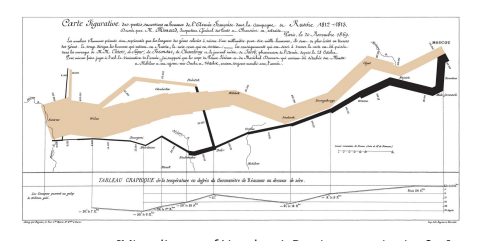
\includegraphics[width=0.5\textwidth]{images/FlowMaps.png}
    \caption{Flow Maps}
    \label{fig:immagine}
\end{figure}
\subsubsection{Chernoff faces}
Ragionamento: siamo molto bravi nel riconoscere i volti.
Introdotto da Herman Chernoff nel 1973
Variabili sono mappate su tratti del viso
(larghezza/curvatura della bocca, dimensione verticale del viso, dimensione/inclinazione/separazione degli occhi, dimensione delle sopracciglia, posizione verticale delle sopracciglia…)
\begin{figure}[H]
    \centering
    \includegraphics[width=0.5\textwidth]{images/Chernofffaces.png} 
    \caption{Chernoff faces}
    \label{fig:immagine}
\end{figure}
\subsubsection{Multidimensional Icons}
Spence e Parr (1991) proposero di codificare le proprietà di un oggetto in una semplice rappresentazione tramite icone. 
Hanno applicato questo approccio per verificare le offerte di permanenza.
\begin{figure}[H]
    \centering
    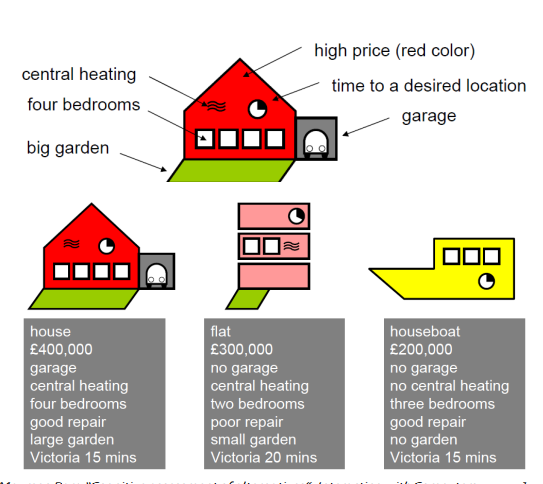
\includegraphics[width=0.5\textwidth]{images/MultiIcon.png} 
    \caption{Multidimensional Icons}
    \label{fig:immagine}
\end{figure}
\subsubsection{Petal as a gliph}
L'idea di Moritz Stefaner per visualizzare un indice di vita consiste nel mappare diverse variabili (relative alle condizioni di vita materiale e alla qualità della vita) in petali di diverse dimensioni, per confrontare il benessere tra paesi.
\begin{figure}[H]
    \centering
    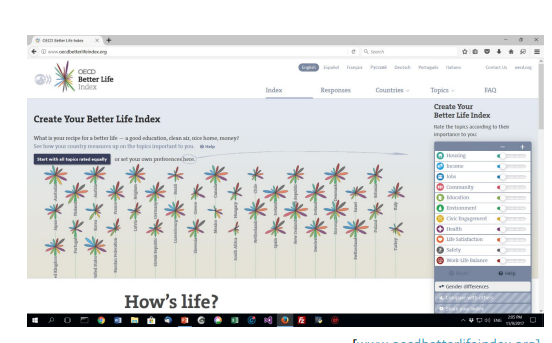
\includegraphics[width=0.5\textwidth]{images/PetalGliph.png} 
    \caption{Petal as a gliph}
    \label{fig:immagine}
\end{figure}


\section{Applied Perception}
Abbiamo visto che la visualizzazione delle informazioni consiste nel trasformare i dati in una rappresentazione 
visuale in modo che un essere umano possa estrarre informazioni utili da essi.
L'\textbf{Effectiveness} di una rappresentazione visuale non è arbitraria: ma dipende fortemente su come funziona il cervello.
Remind: l'efficacia si riferisce alla capacità di una rappresentazione visiva, come un grafico, una mappa o un diagramma, di comunicare in modo chiaro e comprensibile le informazioni desiderate. 
Capire come funziona la percezione può aiutare a prendere decisioni informate riguardo ai design delle visualizzazioni.
L'occhio umano svolge un ruolo fondamentale nella percezione visiva, essendo il principale organo sensoriale che ci consente di interpretare il mondo circostante.
L'\textbf{acuità visiva} è una misura della capacità dell'occhio di distinguere dettagli fini e di percepire chiaramente gli oggetti.
Viene spesso misurata in termini di precisione nella lettura di lettere o simboli su una tavola ottotipica posta a una certa distanza.
La nostra percezione è sensibile al contrasto di pattern, alla frequenza e all'orientamento. Inoltre, il colore influisce sulla funzione del sistema di contrasto spaziale (CSF).
Il visual Cortex è una parte del cervello che gestisce l'elaborazione delle informazioni visive provenienti dagli occhi.
\begin{figure}[H]
    \centering
    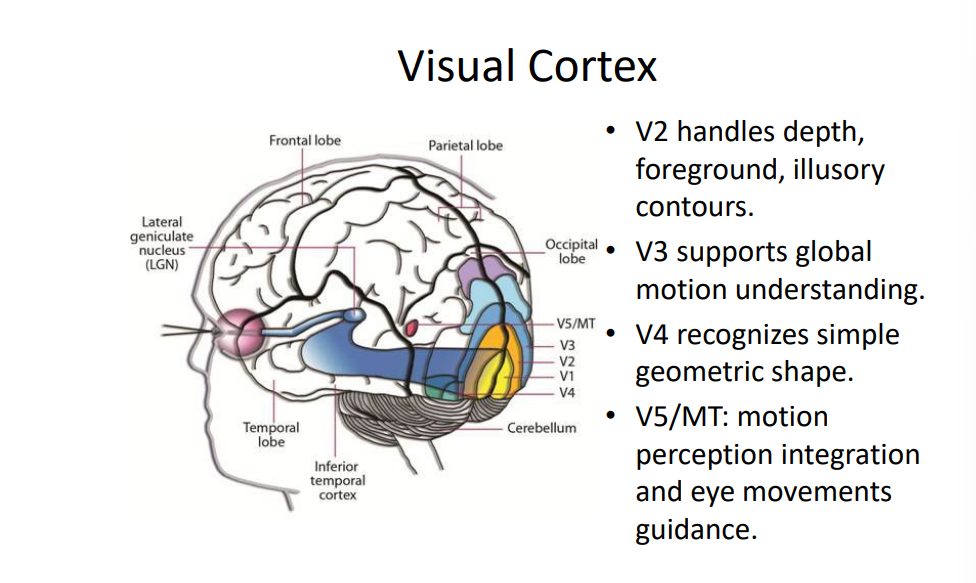
\includegraphics[width=0.5\textwidth]{images/VisualCortex.png} 
    \caption{Divisione del cervello}
    \label{fig:immagine}
\end{figure}
\subsection{Illusions}
Il campo recettivo di una cellula è l'area visiva sulla quale una cellula risponde alla luce.
Le cellule gangliari della retina sono organizzate con campi recettivi circolari.
Quando vengono stimolate al centro, vengono eccitate; quando vengono stimolate al di fuori del centro, vengono inibite.
\subsubsection{Mach Banding}
Le "Mach bands" (bande di Mach) sono un fenomeno ottico che si verifica quando si osservano transizioni tra regioni di luce e ombra su una superficie, creando 
percezioni di contrasto accentuato lungo i confini.
\begin{figure}[H]
    \centering
    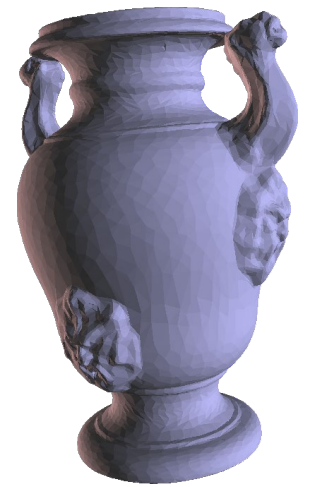
\includegraphics[width=0.5\textwidth]{images/MachBand.png} 
    \caption{Mach Banding}
    \label{fig:immagine}
\end{figure}
\subsubsection{Hermann Grid illusions}

La griglia di Hermann è un'illusione ottica che mette in evidenza l'interazione tra le cellule retiniche e il modo in cui il cervello elabora le informazioni visive. Questa illusione è composta da una griglia di linee grigie disposte a intervalli regolari, 
con dei punti neri posizionati strategicamente agli incroci delle linee.
Si ritiene che l'illusione sia causata dalla percezione del contrasto e dall'inibizione laterale nel sistema visivo. Le cellule retiniche inviano segnali al cervello che possono essere interpretati in modo errato, 
facendo percepire punti ombrosi o grigi nei punti di intersezione delle linee.
\begin{figure}[H]
    \centering
    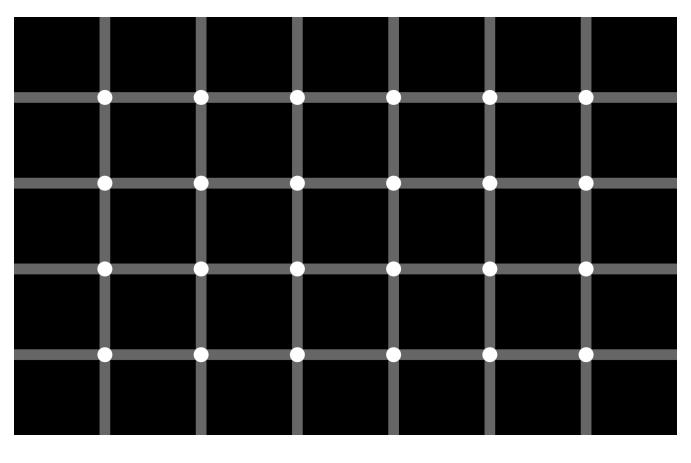
\includegraphics[width=0.5\textwidth]{images/HermmanG.png} 
    \caption{Divisione del cervello}
    \label{fig:immagine}
\end{figure}
\subsubsection{Chevreul Illusion}

L'illusione di Chevreul, chiamata anche illusione dei contrasti simultanei, è un fenomeno ottico che coinvolge la percezione del colore. Questa illusione è dovuta alla sensibilità del nostro sistema visivo ai contrasti e alla relativa interpretazione dei colori circostanti.
Nell'illusione di Chevreul, se viene disegnata una serie di linee parallele in tonalità di grigio simile su uno sfondo bianco, la percezione visiva può far sembrare che i toni di grigio varino lungo le linee. Questo accade a causa dell'interazione tra i colori circostanti e la nostra percezione del contrasto.
Se due tonalità di grigio simili sono separate da una riga più chiara, il grigio sembrerà più scuro del suo vero colore. Al contrario, se sono separate da una riga più scura, sembrerà più chiaro. Questo effetto può far sembrare che i toni di grigio cambino o che vi sia un gradiente lungo le linee parallele,
quando in realtà la differenza di colore non esiste realmente.
 \begin{figure}[H]
    \centering
    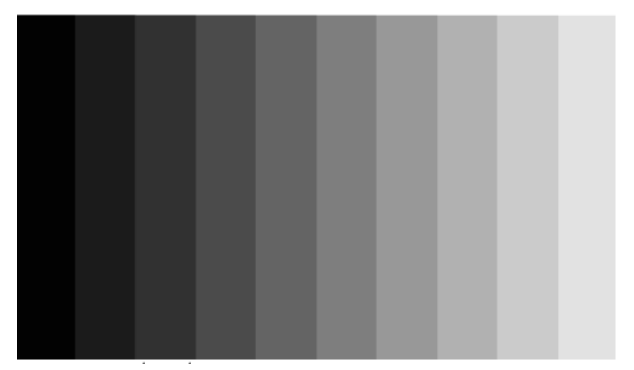
\includegraphics[width=0.5\textwidth]{images/Chevr.png} 
    \caption{Chevreul illusion}
    \label{fig:immagine}
\end{figure}
 \subsubsection{Greyscale Maps}
Questi effetti visivi possono portare a grandi errori quando si leggono informazioni quantitative visualizzate utilizzando una mappa in scala di grigi.
Utilizzare mappe in scala di grigi per rappresentare pochi valori (!)
\subsubsection{The Cornsweet Effect}
Le illusioni di Cornsweet sono un tipo di illusione ottica che evidenzia la percezione umana del contrasto e dei confini tra diverse superfici o tonalità. Questo tipo di illusione si basa sul modo in cui il cervello elabora i cambiamenti graduali di luminosità o colore.
Nell'illusione di Cornsweet, due aree contigue hanno un confine graduale tra loro e una transizione graduale di luminosità o colore. Nonostante la transizione sia graduale e non ci sia un cambiamento netto, la percezione visiva può far 
sembrare che ci sia un confine più netto o un cambiamento repentino.
\begin{figure}[H]
    \centering
    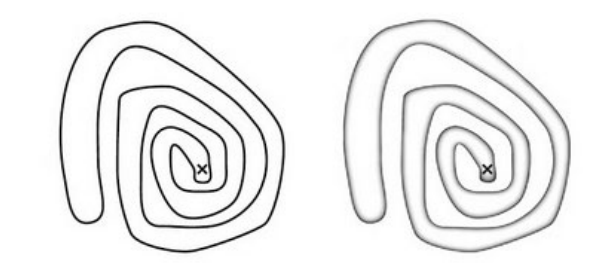
\includegraphics[width=0.5\textwidth]{images/Cornsweet.png} 
    \caption{Cornsweet Effect}
    \label{fig:immagine}
\end{figure}
L'effetto Cornsweet può essere utilizzato per evidenziare regioni delimitate.
Parlando dell'utilizzo delle scale di grigi, in sostanza ci sono delle regole da seguire:
Non utilizzare per mappe o per confrontare molti valori.
Utilizzare per evidenziare:
\begin{itemize}
    \item Regioni delimitate
    \item Elementi importanti (riducendo il contrasto luminoso degli elementi non importanti)
    \item Regolare la luminanza dello sfondo per ottenere una migliore leggibilità.
\end{itemize}
\subsection{Eye Movements}
\textbf{Movimenti oculari:}
\begin{itemize}
    \item \textbf{Movimenti saccadici}: movimenti balistici degli occhi che cambiano il punto di fissazione. Possono essere volontari o scatenati da stimoli.
    \item \textbf{Movimenti di inseguimento lento}: movimenti lenti degli occhi per mantenere uno stimolo in movimento sulla fovea.
    \item \textbf{Movimenti di vergenza}: allineano la fovea di ciascun occhio a un bersaglio in base alla sua distanza.
    \item \textbf{Movimenti vestibolo-oculari}: stabilizzano gli occhi compensando i movimenti della testa.

\end{itemize}
\subsubsection{Preattentive Processes}

I processi preattentivi si riferiscono a quelle operazioni cognitive che avvengono automaticamente e
 istantaneamente nell'elaborazione delle informazioni sensoriali prima che una persona focalizzi la sua attenzione in modo consapevole su di esse. 
 Questi processi avvengono in modo rapido e automatico, senza richiedere uno sforzo cosciente.
Sono responsabili della capacità del cervello di elaborare estrarre informazioni visive, uditiva o tattili in modo veloce ed efficiente. Questi processi sono fondamentali nell'organizzazione delle informazioni sensoriali e possono avvenire a livelli inconsci della percezione umana.
Caratteristiche visive elaborate preattivamente:
\begin{itemize}
    \item Orientamento ; Curvatura ; Forma ; Dimensione ; Colore ;
    Luce/Ombra ; Contenimento ; Concavità/Convessità ;
    \item Alcune di queste non sono simmetriche.
        Caratteristiche visive non elaborate preattivamente:
        Giunzione ; Parallelismo
\end{itemize}
Alcuni processi preattentivi non sono simmetrici:
Aggiungere segni è più efficiente che rimuovere segni.
Aumentare la nitidezza è più efficiente che diminuire la nitidezza.
Un oggetto grande circondato da oggetti piccoli è più efficiente di un oggetto piccolo circondato da oggetti grandi.

\subsubsection{Gestalt Laws}
Le leggi della Gestalt sono principi fondamentali della psicologia della percezione che descrivono come il cervello umano organizza e interpreta le informazioni sensoriali 
per creare una percezione significativa e coerente del mondo che ci circonda. 
\begin{enumerate}
    \item \textbf{Legge della Prossimità}: Gli oggetti vicini tra loro tendono ad essere visti come parte di un insieme o di un gruppo.
    
    \item \textbf{Legge della Similarità}: Gli elementi simili per forma, colore, dimensione o altre caratteristiche tendono ad essere raggruppati insieme nella percezione.
    
    \item \textbf{Legge della Connessione}: Gli oggetti connessi sono percepiti come correlati.
        Collegare diversi oggetti con una linea è un modo efficace per esprimere che esiste una relazione tra di essi.
    
    \item \textbf{Legge della Continuità}: Gli oggetti posti lungo una linea o una curva tendono ad essere visti come parte di un modello o di un flusso continuo.
    
    \item \textbf{Legge della Simmetria}: Gli oggetti disposti simmetricamente sono percepiti come formare un insieme visivo anziché essere considerati entità separate.
     La simmetria è meglio percepita per gli assi orizzontali e verticali.
    
    \item \textbf{Legge della Chiusura}: Le persone tendono a percepire le figure incomplete come forme complete riempiendo le parti mancanti.
    
    \item \textbf{Legge della Simplicità o della Buona Forma}: La percezione tende a organizzare gli stimoli in modo da formare figure semplici e coerenti piuttosto che configurazioni disordinate o complesse.
    
    \item \textbf{Legge della Destinzione Figure-Ground}: Gli oggetti possono essere percepiti come figure distinte rispetto al loro sfondo circostante.
    
    \item \textbf{Legge del Movimento Comune}: Gli oggetti che si muovono nella stessa direzione o seguendo lo stesso modello di movimento possono essere percepiti come parte di un unico oggetto o gruppo.
  \end{enumerate}
  \subsection{Illusions}
  \subsubsection{Muller-Lyer}
  \begin{figure}[H]
    \centering
    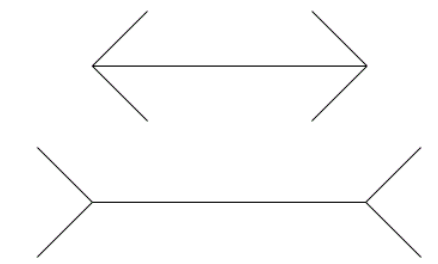
\includegraphics[width=0.5\textwidth]{images/Muller.png} 
    \caption{Muller-Lyer Illusions}
    \label{fig:immagine}
\end{figure}
  Queste due linee hanno lunghezze uguali ma vengono percepite di lunghezze diverse.
    \begin{itemize}
        \item Due spiegazioni:
        \begin{enumerate}
            \item Spiegazione prospettica
            \item Spiegazione del baricentro
        \end{enumerate}
    \end{itemize}
  \subsubsection{Wundt}
  Queste illusioni coinvolgono principalmente la percezione delle dimensioni, delle proporzioni e delle distanze tra gli oggetti, portando
   a percezioni distorte o erronee della realtà visiva.
   \begin{figure}[H]
    \centering
    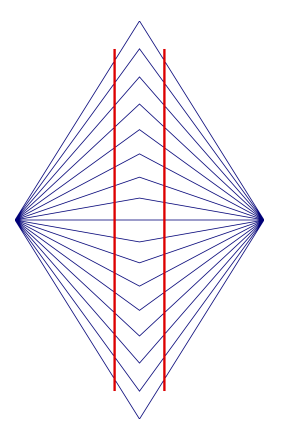
\includegraphics[width=0.5\textwidth]{images/Wundt.png} 
    \caption{Muller-Lyer Illusions}
    \label{fig:immagine}
\end{figure}
  \subsubsection{Hering}
  Un'altra illusione simile (effetto invertito dell'illusione di Wundt).
\begin{itemize}
    \item Possibili spiegazioni:
    \begin{enumerate}
        \item Inibizione laterale
        \item Effetto prospettico
        \item Ritardi temporali nell'elaborazione visiva
    \end{enumerate}
\end{itemize}

  \subsubsection{Horizontal–Vertical Illusion}
  \begin{figure}[H]
    \centering
    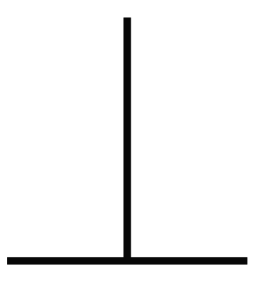
\includegraphics[width=0.5\textwidth]{images/HorizontalVertical.png} 
    \caption{Horizontal–Vertical Illusion}
    \label{fig:immagine}
\end{figure}
  Un'altra semplice illusione scoperta da Wundt.
  La linea verticale viene percepita come lunga al 30\% in più rispetto alla linea orizzontale.
  Sono state osservate differenze (piccole) tra le culture.
  Questo vale anche per le linee che si intersecano.
  \subsubsection{Comparing Area}
  Confrontare le aree è difficile (ricordare le aree dei cerchi appena menzionate).
  \begin{figure}[H]
    \centering
    
\includegraphics[width=0.5\textwidth]{images/Comparing.png} 
    \caption{Comparing Area}
    \label{fig:immagine}
\end{figure} 
    \begin{itemize}
        \item Quando confrontiamo le aree, le proporzioni sono sottovalutate (peggio per i volumi).
        \item Flannery (1970) propose di compensare la percezione applicando un fattore di scala percettiva.
        \item Tufte, nel suo famoso libro "The Visual Display of Quantitative Information" (2001), si oppose a qualsiasi cosa tranne che l'uso di una scala assoluta, ovvero esclude la compensazione per le mancanze percettive umane.
    \end{itemize}
    La scalatura percettiva potrebbe essere insufficiente. Le cose sono più complesse da un punto di vista percettivo
\subsubsection{Weber's Law}
Ernst Heinrich Weber (1795 1878) ha condotto studi sulla percezione degli stimoli fisici da parte dei sensi umani (visione, udito, gusto, tatto e olfatto).
Legge di Weber: \\
$ \frac{\Delta S}{S}=K $ \\

Legge di Weber:
\begin{itemize}
    \item La percezione dipende dallo stimolo iniziale.
    \item  I rapporti sono più importanti dei valori assoluti.
\end{itemize}


\section{Applied Perception II }
\subsection{Color Vision}
La \textit{Color Vision} può essere considerata come superflua nella vita moderna
Ma il colore comunque è estreamamente utile nella data visualization:
\begin{itemize}
    \item Mostrare i patterns
    \item Labeling
    \item Mettere in evidenza
\end{itemize}
\begin{figure}[H]
    \centering
    \begin{minipage}{0.45\textwidth}
        \centering
        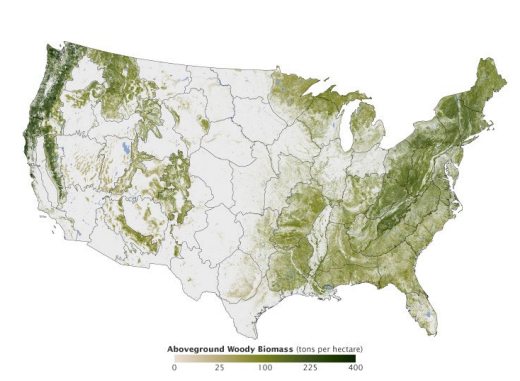
\includegraphics[width=\linewidth]{images/ColorVision.png} 
        \caption{Effetti della color vision}
        \label{fig:immagine1}
    \end{minipage}\hfill
    \begin{minipage}{0.45\textwidth}
        \centering
        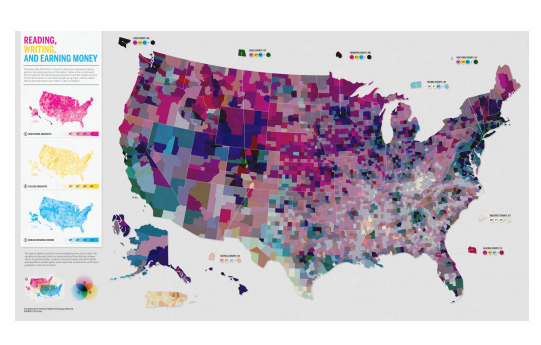
\includegraphics[width=\linewidth]{images/ColorVision2.png} 
        \caption{Effetti della color vision}
        \label{fig:immagine2}
    \end{minipage}
\end{figure}
Pensare al colore come un attributo di un oggetto invece che ad una caratteristica primaria(C.Ware).
\subsection{Trichromacy and Opponent process theories}
Abbbiamo, sulla retina, tre distinti recettori per i colori:
\begin{itemize}
    \item the \textbf{cones}: che sono attivi ai livelli normali di luce
    \item the \textbf{rods}: l'influenza dei rods sulla percezione può essere ignorata.
\end{itemize}
\subsubsection{Trichromacy theory}
I \textit{cones} sono sensibili alle diverse onde di luce.
Quindi, assorbono luce attorno lo spettro del colore blue, verde e rosso.
La teoria dice che percepiamo il colore tramite un sistema a tre canali.
Tutti gli spazi dei colori, anche se progettati per scopi diversi, sono tridimensionali.
\begin{figure}[H]
    \centering
    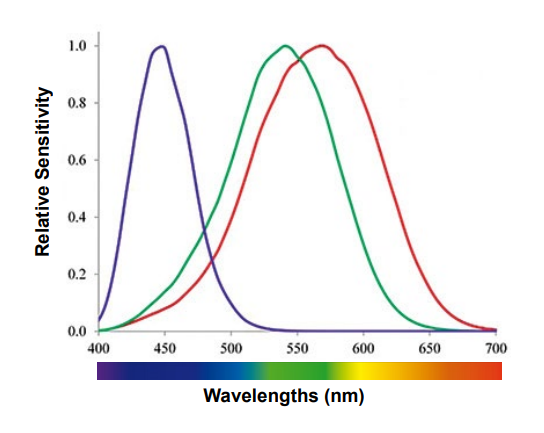
\includegraphics[width=0.5\textwidth]{images/Thrichromacy.png} 
    \caption{Trichromacy theory}
    \label{fig:immagine}
\end{figure}
\subsubsection{colour measurement and specifcation}
Dato che solo tre diversi recettori sono coinvolti nella colori vision, è possibile fare il match dei colori
usando un mix di tre colori, chiamati primari.
Dato uno standard di colori primari, si può usare una transformazione per creare lo stesso colore in output in device diversi 
\begin{figure}[H]
    \centering
    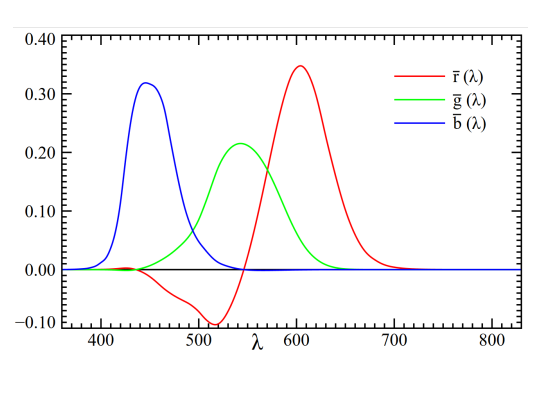
\includegraphics[width=0.5\textwidth]{images/RGB.png} 
    \caption{RGB color Matching Function}
    \label{fig:immagine}
\end{figure}
\subsubsection{CIE XYZ Color Space}

Lo spazio colore CIE XYZ è uno spazio colore standardizzato sviluppato dalla Commission Internationale de l'Eclairage (CIE). È un modello matematico che rappresenta tutti i colori visibili agli esseri umani attraverso tre valori numerici: X, Y e Z.
Questi valori sono definiti in base alle risposte dei tre tipi di coni presenti nell'occhio umano (sensibili alle lunghezze d'onda dei colori rosso, verde e blu).
Il valore Y rappresenta la luminosità, mentre X e Z descrivono la posizione orizzontale e verticale del colore nello spazio XYZ.
 
Il diagramma di cromaticità è uno strumento visivo utilizzato per rappresentare i colori visibili senza tener conto della luminosità. Questo diagramma rappresenta le proprietà del colore in termini di tonalità e saturazione, ignorando la luminanza.
\subsubsection{Opponent process theory}

Alla fine del XIX secolo, il psicologo tedesco Hering propose la teoria (successivamente supportata da prove sperimentali) secondo cui i coni della retina combinano il loro stimolo formando tre coppie di colori che competono tra loro per formare quello finale. Queste coppie, chiamate coppie antagoniste, sono: nero-bianco, giallo-verde e giallo-blu
\textbf{Evidenze a supporto della teoria:}
\begin{itemize}
  \item Nomenclatura
  \item Tonalità uniche
  \item Neurofisiologia
\end{itemize}

\textbf{Proprietà dei canali di colore antagonisti:}
\begin{itemize}
  \item Risoluzione spaziale
  \item Percezione della forma
  \item Contrasto cromatico
\end{itemize}

La teoria della tricromia e la teoria dei colori antagonisti operano a livelli differenti.

La teoria della tricromia spiega ciò che accade a livello dei fotorecettori.
La teoria dei colori antagonisti spiega ciò che accade a livello neurale.
\subsection{Color Space}
\subsubsection{RGB Color Space}

Lo spazio dei colori \textbf{RGB} (Red, Green, Blue) è un modello di colore utilizzato comunemente nel contesto digitale e dell'informatica per rappresentare i colori. Questo spazio dei colori si basa sulla combinazione di tre colori primari: rosso (Red), verde (Green) e blu (Blue).
Nel modello RGB, ogni colore può essere rappresentato come una combinazione di intensità di questi tre colori primari. Ogni colore è rappresentato da un punto in uno spazio tridimensionale dove i tre assi corrispondono a rosso, verde e blu.
La combinazione di diverse intensità di rosso, verde e blu consente di ottenere una vasta gamma di colori. Ad esempio, il nero si ottiene quando tutte e tre le componenti (R, G, B) sono al minimo, mentre il bianco si ottiene quando tutte e tre
 sono al massimo. I colori primari (rosso, verde e blu) sono usati come base per creare tutti gli altri colori nel modello RGB.
\begin{figure}[H]
    \centering
    \includegraphics[width=0.5\textwidth]{images/RGBCOlor.png} 
    \caption{RGB color}
    \label{fig:immagine}
\end{figure}
\subsubsection{HSV/HSL color space}

\textbf{HSV} (Hue, Saturation, Value) e \textbf{HSL} (Hue, Saturation, Lightness) sono due modelli di spazio dei colori correlati che rappresentano i colori in termini di tre componenti principali: tonalità (Hue), saturazione (Saturation) e valore o luminosità (Value per HSV, Lightness per HSL).
La specifica del colore risulta essere più intuitiva con HSV/HSL rispetto a RGB. Tuttavia, questi spazi di colore non sono uniformi dal punto di vista percettivo, il che implica che le distanze calcolate all'interno dello spazio colore 
non corrispondono alle distanze percettive.
\subsubsection{CIE Lab/Lch color space}
Lo spazio colore CIE Lab/Lch è un sistema di colore sviluppato dalla Commissione Internazionale dell'Illuminazione (CIE). Questo spazio colore è progettato per rappresentare i colori in modo più uniforme e vicino alla percezione umana rispetto ad altri spazi 
colore come RGB, HSV o HSL.
\subsubsection{Color differences}
Avere uno space color in cui le distanze percettive uguali corrispondono a distanze uguali è utile per specificare tolleranze del colore, codici colore, pseudocolore (utilizzando sequenze di colori per rappresentare valori dei dati, possibilmente con passaggi percettivamente uguali).
Anche se gli space color uniformi forniscono solo un'approssimazione iniziale approssimativa di come saranno percepite le differenze di colore, un fattore influente importante è la dimensione (siamo molto più sensibili alle differenze tra grandi campi).
Suggerimento: utilizzare colori saturi quando si codifica piccoli simboli o linee sottili e colori meno saturi per aree grandi.
\begin{figure}[H]
    \centering
    \includegraphics[width=0.5\textwidth]{images/ColorDifferences.png} 
    \caption{Color differences}
    \label{fig:immagine}
\end{figure}
\subsection{Color and visualization}
\subsubsection{Luminance and visualization}
I canali cromatici rosso-verde e giallo-blu sono in grado ciascuno di trasportare 
solo circa un terzo della quantità di dettagli trasportati dal canale in bianco e nero (Mullen, 1985). 
Le differenze puramente cromatiche non sono sufficienti per visualizzare dettagli fini. Assicurare un adeguato contrasto di luminanza con lo sfondo (anche se vengono utilizzati colori con differente cromaticità).
Un confine di contrasto può migliorare la leggibilità dei simboli colorati.
\subsubsection{Saturation and visualization}
Utilizzare colori saturi per codificare piccoli simboli/dettagli fini e colori meno saturi per codificare aree grandi.
\subsubsection{Color for Labeling}
Post e Greene (1986) hanno condotto un esperimento sulla denominazione dei colori (sono stati mostrati 210 colori diversi su uno sfondo nero in una stanza oscurata). Solo otto colori più il bianco vengono denominati in modo coerente. Anche se non è generalmente applicabile,
ciò suggerisce che solo pochi colori possono essere utilizzati come etichette di categoria.
\subsubsection{Color and semantics}
Fai attenzione alle convenzioni dei colori e alle associazioni semantiche (rosso per caldo/cattivo/pericolo, blu per freddo, verde per vita/vai, ecc.), 
poiché le convenzioni non sono universali. L'associazione semantica con il grigio è quella di appartenenza a una categoria non specificata (utile per evidenziare)
Evita colori problematici per le persone daltoniche.
Utilizza una scala di colori basata sullo spettro solo quando il suo utilizzo è profondamente radicato nella cultura degli utenti.
Per rivelare dettagli fini, utilizza sequenze di pseudocolori che variano nella luminosità, non solo nella cromaticità.

\end{document}